% Copyright 2021 Edoardo Riggio

% Licensed under the Apache License, Version 2.0 (the "License");
% you may not use this file except in compliance with the License.
% You may obtain a copy of the License at

% 	http://www.apache.org/licenses/LICENSE-2.0

% Unless required by applicable law or agreed to in writing, software
% distributed under the License is distributed on an "AS IS" BASIS,
% WITHOUT WARRANTIES OR CONDITIONS OF ANY KIND, either express or implied.
% See the License for the specific language governing permissions and
% limitations under the License.

\documentclass{article}

\usepackage{hyperref, amsmath, graphicx, amssymb}
\usepackage{fancyvrb,newverbs,xcolor}

\graphicspath{ {./assets/} }

\definecolor{cverbbg}{gray}{0.93}

\newenvironment{cverbatim}
 {\SaveVerbatim{cverb}}
 {\endSaveVerbatim
  \flushleft\fboxrule=0pt\fboxsep=.5em
  \colorbox{cverbbg}{\BUseVerbatim{cverb}}%
  \endflushleft
}

\newenvironment{lcverbatim}
 {\SaveVerbatim{cverb}}
 {\endSaveVerbatim
  \flushleft\fboxrule=0pt\fboxsep=.5em
  \colorbox{cverbbg}{%
    \makebox[\dimexpr\linewidth-2\fboxsep][l]{\BUseVerbatim{cverb}}%
  }
  \endflushleft
}

\newcommand{\ctexttt}[1]{\colorbox{cverbbg}{\texttt{#1}}}
\newverbcommand{\cverb}
  {\setbox\verbbox\hbox\bgroup}
  {\egroup\colorbox{cverbbg}{\box\verbbox}}

\begin{document}
\begin{titlepage}
    \begin{center}
        \vspace*{1cm}
        
        \Huge
        \textbf{Information Retrieval Cheatsheet}
        
        \vspace{0.5cm}
        \LARGE
        
        \vspace{.5cm}
        
        Edoardo Riggio
   		  \vspace{1.5cm}
       
        \vfill
        
        \today
        
        \vspace{.8cm}
          \Large
          Operating Systems - SA. 2021 \\
        Computer Science\\
        Universit\`{a} della Svizzera Italiana, Lugano\\
        
    \end{center}
\end{titlepage}

\tableofcontents

\newpage

\section{Introduction}
\subsection{Text Information Systems}
Text Information Systems involve three main capabilities:

\begin{itemize}
	\item Text Retrieval
	\vspace{.2cm} \\
	Information Retrieval is a field concerned with the structure, analysis, organization, storage searching, and retrieval of information.
	
	\item Text Analysis
	\vspace{.2cm} \\
	Analyze large amounts of text data in order to discover interesting patterns buried in text.
	
	\item Text Organization
	\vspace{.2cm} \\
	Annotate a collection of text documents with meaningful topical structures so that scattered information can be connected and navigated.
\end{itemize}
While text retrieval is part of information retrieval, text analysis and text organization are part of text mining. \\ \\
Differently from queries done on DBMS, queries in search engines make use of natural language. It is much harder to compare the text query to the document text and determining what is a good match and what is not a good match. This is the core issue of information retrieval. There are many different ways of writing the same thing, thus an identical matching of words is not enough.

\subsection{Relevance}
A document is said to be relevant when it contains the information that a person was looking for when he/she submitted the query tot eh search engine.\\ \\
In order to understand what the user is asking for in the query, we use something that is known as \textbf{NLP} (Natural Language Processing). NLP is concerned with developing techniques for enabling computers to understand the meaning of natural language text.

\section{Text Access}
Text data access is the foundation for text analysis. The general goal of text data access is to connect users with the right information at the right time. \\ \\
Connection with users can be done in two ways:

\begin{itemize}
	\item \textbf{Pull}
	\vspace{.2cm} \\
	The user takes initiative in order to fetch relevant information from the system.
	
	\item \textbf{Push}
	\vspace{.2cm} \\
	The system takes initiative in order to offer relevant pieces of information to the users.
\end{itemize}

\subsection{Access Mode: Pull vs Push}
In \textbf{pull} mode, the user initiates the access process in order to find the relevant text data. When a user has such need, then this can be done in two different ways:

\begin{itemize}
	\item \textbf{Querying}
	\vspace{.2cm} \\
	The user can use a query in order to obtain ad hoc information. This mode of research is done by using a few -- yet specific -- words.
	
	\item \textbf{Browsing}
	\vspace{.2cm} \\
	It is a way of accessing text data, and can be very useful for users when they do not know how to formulate an effective query.
\end{itemize}
In \textbf{push} mode, the system initiates the process to recommend a set of relevant information items to the user. \\ \\
Broadly, there are two kinds of information needs:

\begin{itemize}
	\item \textbf{Short-Term Needs}
	\vspace{.2cm} \\
	These needs are often associated with pull mode. This type of information need is temporary and usually satisfied through searching or browsing.
	
	\item \textbf{Long-Term Needs}
	\vspace{.2cm} \\
	These needs are often associated will pull mode. This type of information need can be better satisfied through filtering or recommendation of the system to the user.
\end{itemize}
Finally we have \textbf{browsing traces}. These traces happen whenever a user does any kind of browsing. They are used in order to model the behaviour of the user, and make more precise recommendations.

\subsection{Search Engine Architecture}
A \textbf{software architecture} consists of software components, the interfaces provided by those components, and the relationships between them. \\ \\
The software architecture of a search engine is determined by the following requirements:

\begin{itemize}
	\item \textbf{Effectiveness}
	\item \textbf{Efficiency}
\end{itemize}
An information retrieval process can be divided into four subprocesses:

\begin{enumerate}
	\item \textbf{Indexing Process}
	\vspace{.2cm} \\
	This process is composed of several different stages. First we have \textbf{text acquisition}, in which the system identifies and stores documents for indexing. \\ \\
	Second we have \textbf{text transformation}, in which the system transforms documents into index terms or features. \\ \\
	Finally we have \textbf{index creation}, in which the system takes index terms and creates data structures to support fast searching.
	
	\item \textbf{Query and Retrieval Process}
	\vspace{.2cm} \\
	It is composed of the following stages. \textbf{User interaction}, which supports the creation of a query and displays the results. \\ \\
	Next we have \textbf{ranking and retrieval}, in which the query and indices are used in order to generate a ranked list of documents. \\ \\
	Finally we have \textbf{evaluation}, which monitors and measures the effectiveness and efficiency of the information retrieval system.
	
	\item \textbf{Relevance Feedback Process}
	\vspace{.2cm} \\
	It is composed of three parts. The first part is the \textbf{user evaluation}, where the user assesses the effectiveness of the system. \\ 
	Then we have \textbf{user feedback}, which supports refinement of the query and display of the result.\\
	Finally we have \textbf{ranking and retrieval}, where the system generates a ranked list of the documents.
\end{enumerate}

\subsection{Formal Definition of Information Retrieval}
Information retrieval is composed of several elements, such as:

\begin{itemize}
	\item \textbf{Vocabulary}
	\vspace{.2cm} \\
	Vocabulary is defined as:
	\[ V = \{ w_1, w_2, ..., w_n \} \]
	This represents the vocabulary of a language.
	
	\item \textbf{Document}
	\vspace{.2cm} \\
	A document is defined as:
	\[ d_i = d_{i1}, ..., d_{iM} \]
	Where $d_{ij} \in V$.
	
	\item \textbf{Collection}
	\vspace{.2cm} \\
	A collection is defined as:
	\[ C = \{d_1, ..., d_M\} \]
	this represents a collection of documents.
	
	\item \textbf{Query}
	\vspace{.2cm} \\
	A query is defined as:
	\[ q = q_1, ..., q_M \]
	Where $q_j \in V$.
	
	\item \textbf{Relevant Documents}
	\vspace{.2cm} \\
	This set is defined as:
	\[ R(q) \subseteq C \]
	And it is generally unknown and user-dependent. The query acts as a hint on which the document must be contained in $R(q)$.
\end{itemize}

\subsection{How to Compute $R'(q)$}
$R'(q)$ can be computed in one of two ways:

\begin{itemize}
	\item \textbf{Document Selection}
	\vspace{.2cm} \\
	This can be described as:
	\[ R'(q) = \{ d \in C~|~f(d, q) = 1 \} \]
	Where $f(d, q) \in \{0,1\}$ and is an indicator function/binary classifier. Here the system must decide whether a document is relevant or not -- i.e. \textbf{absolute relevance}. This is also known as \textbf{boolean retrieval}.
	
	\item \textbf{Document Ranking}
	\vspace{.2cm} \\	
	This can be defined as:
	\[ R'(q) = \{ d \in C~|~f(d,q) > \Theta\} \]
	Where $f(d,q) \in \mathbb{R}$ is a relevance measure function, and $\Theta$ is a cutoff determined by the user. Here the system only decides if one document is more likely relevant than another -- i.e. \textbf{relative measure}. This is also known as \textbf{ranked retrieval}.
\end{itemize}

\section{Implementation of an IR System}
An information retrieval system is mainly made up of four components:

\begin{enumerate}
	\item \textbf{Tokenizer}
	\vspace{.2cm} \\
	This component takes in documents as raw strings and determines how to separate the large document into separate tokens.
	
	\item \textbf{Indexer}
	\vspace{.2cm} \\
	This module processes documents and indexes them with appropriate data structures. This module can be ran offline.
	
	\item \textbf{Scorer/Ranker}
	\vspace{.2cm} \\
	This module takes a query and returns a ranked list of documents.
\end{enumerate}

\subsection{Indexing}
The main role of the indexer is to convert documents into data structures in order to enable fast search. The \textbf{inverted index} is the dominant indexing method for supporting basic search algorithms. \\ \\
This data structure is composed of two parts:

\begin{itemize}
    \item \textbf{Lexicon}
	\vspace{.2cm} \\
	It is a table of search-specific information, such as document frequency and where to find in the postings the per-document term counts
	
	\item \textbf{Posting File}
	\vspace{.2cm} \\
	It is a mapping that goes from any term integer ID to a list of documents IDs and frequency information of the term in those documents.
\end{itemize}
Before obtaining the inverted index we need to pre-process the documents in order to extract only the features we are interested in.

\subsection{Zipf's Law}
The distribution of words in documents is very skewed. This means that only a few words occur often, while many other words occur rarely. \\ \\
Zipf's Law says that the rank $r$ of a word times its frequency $f$, is approximately a constant $k$ -- assuming that the words are ranked in decreasing order of frequency. Thus we have the following formula:
\[ r \cdot f \approx k \] \\
In the following case, for example, the words on the far right -- with $x = [0, 7.5)$ -- are high frequency words, thus useless, the words in the middle -- with $x = [7.5, 15)$ -- are intermediate frequency words, thus very useful, and the words in the far right -- with $x = [15,25]$ -- are rare words, thus they might be useful. \\ \\

\begin{center}
	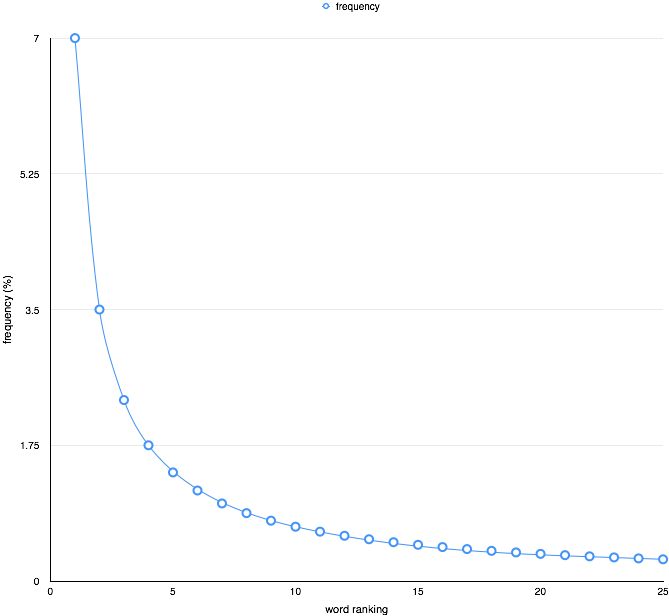
\includegraphics[width=7cm]{zipf.png}
\end{center}

\subsection{Text Indexing}
Text indexing can be divided into the following steps:

\begin{enumerate}
	\item \textbf{Tokenization}
	\item \textbf{Stopword Removal}
	\item \textbf{Stemming}
	\item \textbf{Detecting Phrases}
	\item \textbf{POS Tagging and N-Grams}
	\item \textbf{Processing Document Structure and Markup}
	\item \textbf{Named Entity Recognition}
	\item \textbf{Link Analysis}
	\item \textbf{Build the Inverted Index}
	\item \textbf{Compress the Inverted Index}
\end{enumerate}

\subsubsection{Tokenizing}
To tokenize means to break down words into appropriate sequences of characters. \\ \\
The first step is to use the \textbf{parser} in order to identify the appropriate parts of the document that need to be tokenized.

\subsubsection{Stopping Removal}
Some words have little to no meaning on their own and occur very frequently. These are treated as stopwords and removed. Although, sometimes, they could be important in combination with other words.

\subsubsection{Stemming}
Many morphological variations of words exist. In most cases, these have the same or very similar meanings. The goal of \textbf{stemmers} is to attempt to reduce morphological variations of words to a common stem. \\ \\
For example, the words \textit{consign}, \textit{consigned}, \textit{consigning} and \textit{consignment} can all be reduced down to \textbf{consign}. \\ \\
There are two main types of stemming approaches:

\begin{itemize}
	\item \textbf{Algorithmic Approach}
	\vspace{.2cm} \\
	In this case it is a program that determines related words. This could give some false positives and many false negatives.
	
	\item \textbf{Dictionary-Based Approach}
	\vspace{.2cm} \\
	In this case a list of related words is used. Endings are removed based on a dictionary. This approach produces real words, not stems, and it's much more precise -- but more expensive to run.
\end{itemize}
Some used stemmers are:

\begin{itemize}
	\item \textbf{Porter Stemmer}
	\vspace{.2cm} \\
	This is an algorithm used since the 70s. It consists of a series of rules designed to remove the longest possible suffix from a word at each step. It produces stems, not real words. Sometimes this algorithm can be too aggressive or too weak. Porter2 stemmer was created in order to address some of the issues Porter had.
	
	\item \textbf{Krovertz Stemmer}
	\vspace{.2cm} \\
	This is a hybrid algorithmic-dictionary stemmer. The word is checked in a dictionary. If the word is present, then the word is either left alone or replaced with "exception", if the word is not present, the word is checked for suffixes that could be removed. Finally, after the removal, the dictionary is checked again. \\ \\
	In this case words are generated, not stems. Furthermore, this stemmer has lower false positives, but higher false negatives.
\end{itemize}

\subsubsection{POS Tagger and N-Grams}
\textbf{POS (Part Of Speech) tagging} is the process of marking up a word in a text as corresponding to a particular part of speech, based on both its definition and its context. POS taggers use statistical models of text in order to predict syntactic tags of words. \\ \\
Since POS tagging is too slow for some collections, \textbf{N-Grams} also exist. These are typically formed from overlapping sequences of words. Frequent N-Grams are more likely to be useful phrases. N-Grams follow Zipf's distribution.

\subsubsection{Build the Inverted Index}
In order to construct an inverted index, we use sort-based methods by following these steps:

\begin{enumerate}
	\item Collect local tuples, such as term IDs, Doc IDs and frequency;
	\item Sort the local tuples;
	\item Perform pair-wise merge runs;
	\item Output the inverted file.
\end{enumerate}
While the dictionary part of the inverted index is of modest size, the postings part is huge and stored on disk.

\subsection{Ranking Documents}
The formula that is used in order to rank documents is the following.
\[ f(q, d) = f_a (h (g (t_1, d, q), ..., g (t_k, d, q)), f_d(d), f_q(q)) \]
Where $f_d(q)$ and $f_q(q)$ are pre-computed. Moreover, a score accumulator is maintained for each $d$ in order to compute $h$. Finally, for each query term $t_i$, the following inverted list is fetched.
\[ \{ (d_1, f_1), ..., (d_n, f_n) \} \]
In order to improve the efficiency of the ranker, one could use caching, and keep only the most promising accumulators. There is no need for parallel processing.

\section{Retrieval Models}
The retrieval process is based on a retrieval model which matches a query with a document. There are at least two classes of retrieval models:

\begin{itemize}
	\item \textbf{Set-Based Models}
	\vspace{.2cm} \\
	These are models like the Boolean model, and are defined by the following function:
	\[ f(q, d) = \{ 0,1 \} \]
	
	\item \textbf{Similarity-Based Models}
	\vspace{.2cm} \\
	These are models such as the vector space model, the probabilistic model... They are defined by the following function:
	\[ f(q,d) = \text{similarity}(q, d) = [0, \infty) \]
\end{itemize}

\subsection{Examples of Retrieval Models}
\subsubsection{Boolean Model}
A boolean model can only have two possible outcomes for query processing: true or false. It is an exact-match retrieval process, and the simplest for of ranking. \\ \\
A query is usually specified using boolean operators (such as AND, NOT, OR...), and is used in DBMSs. \\ \\
Some advantages of boolean retrieval are:

\begin{itemize}
	\item The result is predictable;
	\item Many different features can be incorporated;
	\item Efficient query processing.
\end{itemize}
While the disadvantages are:

\begin{itemize}
	\item The effectiveness of the query solely depends on the user;
	\item Simple queries do not usually work well;
	\item Complex queries are difficult both to think and to write.
\end{itemize}

\subsubsection{Ranked Retrieval}
In ranked retrieval, documents are presented according to how much they match the query. In a good ranking function relevant documents should be ranked on top of non-relevant ones.

\subsection{Designing Retrieval Models}
All retrieval models are based on the assumption of using a \textbf{bag-of-words} representation of text. A bag-of-words is a model in which a text is represented as the multiset of its words, disregarding grammar and even word order. \\ \\
In order to design a retrieval function, we require a computational definition of relevance. Moreover, we need to use features such as:

\begin{itemize}
	\item \textbf{Term Frequency (TF)}
	\vspace{.2cm} \\
	This represents how many times does one term appear inside of each document.
	
	\item \textbf{Document Length}
	\vspace{.2cm} \\
	If a term occurs in a long document many times, it is not as significant as a term that occurs the same number of times inside a short document.
	
	\item \textbf{Document Frequency (DF)}
	\vspace{.2cm} \\
	This represents how often a term appears at least once in any document of the entire collection.
\end{itemize}

\subsection{Vector Space Model}
This is a simple, yet effective, way of designing ranking functions for information retrieval systems. This is a special case of similarity-based models, where we assume that relevance is roughly correlated to the similarity between a query and a document. \\ \\
In this representation, each dimension of a highly dimensional space represents a term. We can plot the documents in the collection as vectors of term magnitude.

\begin{center}
	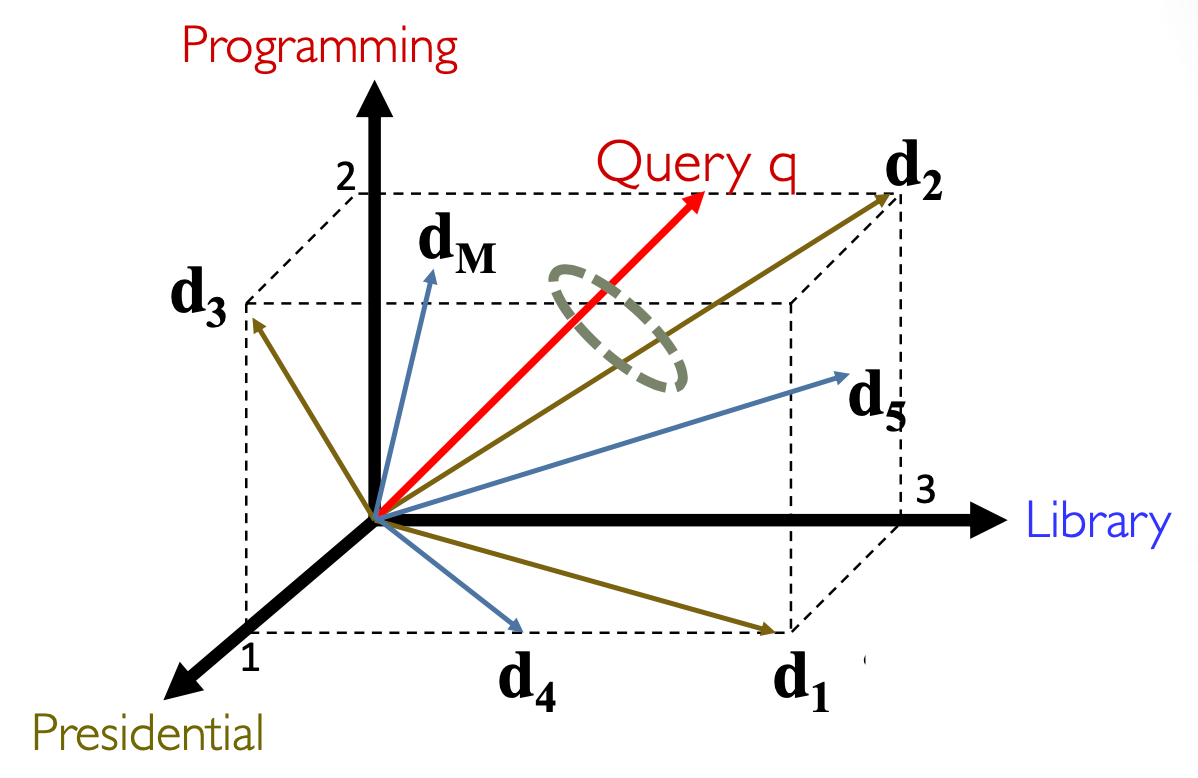
\includegraphics[width=9cm]{vsm.png}
\end{center}
This is a framework, thus it needs to be defined. In order to use this framework we need the following:

\begin{itemize}
	\item \textbf{Dimension Instantiation}
	\vspace{.2cm} \\
	The number of dimension can be defined by the number of words inside of a bag-of-words.
	
	\item \textbf{Vector Placement}
	\vspace{.2cm} \\
	In order to place the vector inside of the framework, we can use bit vectors. These bit vectors can only be either 0 or 1. We will have a 1 if the word $w_i$ -- one of the words of the axes -- is present in the document or query, 0 otherwise.
	
	\item \textbf{Similarity Instantiation}
	\vspace{.2cm} \\
	The similarity between a query and a document can be defined as the dot product between these two vectors. In this case the formula would be:
	\[ \text{sim}(q, d) = \langle q, d \rangle = \sum^N_{i = 1} x_i \cdot y_i \]
\end{itemize}
By using only these definitions and instantiations, the framework will be limited. For example, wouldn't it be correct to give more credit to terms that appear more times in a document or query? The current model does not allow it. This is why we can introduce some improvements to the current model, such as:

\begin{itemize}	
	\item \textbf{Term Frequency Vector}
	\vspace{.2cm} \\
	An improvement can be applied by representing a frequency vector. This vector will represent the number of times that the word $w_i$ -- one of the words of the axes -- is contained in the query or in the document.
	
	\item \textbf{Term Frequency Weighting (TFW)}
	\vspace{.2cm} \\
	This improvement consists in using the same formula as the one used in the similarity instantiation, but with $q$ and $d$ represented by term frequency vectors.
	
	\item \textbf{Inverse Document Frequency}
	\vspace{.2cm} \\
	This improvement consists in giving a weight to words. The formula for computing $y_i$ is given by:
	\[ y_i = \text{count}(w_i, q) * \log \left( \frac{M+1}{k} \right) \]
	Where $\text{count}(w_i, q)$ is the number of times the word $w_i$ appears in document $d$, $M$ is the total number of documents in a collection, and $k$ is the total number of documents containing the word $w$. \\ \\
	The weight of each word inside of the collection of documents is computed by the second part of the previous formula, i.e.
	\[ \log \left( \frac{M+1}{k} \right) \]
\end{itemize}

\subsubsection{TF Transformation}
Since the inverse document frequency still has some problems, we can use TF transformation in order to normalize the number of times a word appears in a collection. This method is used in order to avoid the dominance of a single term above all the others. \\ \\
This transformation, is mathematically defined as follows:

\[ f(q, d) = \sum_{w \in q \cap d} \text{count}(w, q) \cdot \frac{(k+1) \cdot \text{count}(w, d)}{\text{count}(w, d) + k} \cdot \log \left( \frac{M+1}{df(w)} \right) \]
Where $k \geq 0$ is a constant, $w \in q \cap d$ indicates all matched query words in the document, and $df(w)$ indicates the document frequency of the word $w$.

\subsubsection{Document Length Normalization}
Since a long document has a higher chance of matching any query, it must be penalised -- but not too much -- by using a document length normalizer. In order to not over-penalise a long document, we say that a document with more words must be penalised more, while a document with more contents must be penalised less. \\ \\
In order to normalize the document lengths, we use the average document length as a pivot. The formula of the document length normalizer is the following:
\[ 1 - b + b \cdot \left( \frac{|d|}{\text{avgdl}} \right) \]
Where $b \in [0, 1]$ is a constant and \textit{avgdl} is the average length of the documents in the collection.

\subsection{Probabilistic Models}
In probabilistic models, we define the ranking function based on the probability that a given document $d$ is relevant to a query $q$.
\[ p(R = 1~|~d,q) \]
Where $R \in \{ 0,1 \}$ is a binary random variable that denotes relevance. In order to define relevance in a model such as this, we use the following formula.
\[ p(R=1~|~q,d) = \frac{\text{count}(R=1, d,q)}{\text{count}(d,q)} \]

\subsection{Query Likelihood Retrieval Model}
In query likelihood models, our assumption is that the probability of relevance can be approximated by the probability of a query given a document and a relevance.
\[ p(q~|~d, R=1) \]
This captures the following probability: if a user likes document $d$, how likely would the user enter query $q$ in order to retrieve document $d$? In this model we assume that the user imagines some ideal document, and generates a query based on that ideal document.

\subsection{Statistical Language Model}
A statistical language model is used in order to compute the probability of text. For example:

\begin{align*}
	p(\text{\textit{"Today is Wednesday"}}) & \approx 0.001 \\
	p(\text{\textit{"Today Wednesday is"}}) & \approx 0.0000000000001 \\
	p(\text{\textit{"The eigenvalue is positive"}}) & \approx 0.00001
\end{align*} \\
This probability distribution over word sequences is highly context- and user-dependent. This is also called a generative model. \\ \\
Language model is useful to quantify the uncertainties in natural language. It can be particularly useful in:

\begin{itemize}
	\item \textbf{Speech Recognition}
	\item \textbf{Text Categorization}
	\item \textbf{Information Retrieval}
\end{itemize}

\subsubsection{Unigram Language Model}
Unigram language model is the simplest form of a language model. It generates text by generating each word independently. Thus:
\[ p(w_1, w_2, ..., w_n) = p(w_1) + p(w_2) + ... + p(w_n) \]
In order to compute a more accurate estimation of unigrams, we could use topic representation. To do so we get:

\begin{itemize}
	\item \textbf{Background Language Model}
	\vspace{.2cm} \\
	This LM is composed of terms contained in a general background English text. Mathematically this is equal to:
	\[ p(w~|~B) \]
	
	\item \textbf{Topic Language Model}
	\vspace{.2cm} \\
	This LM is composed of terms contained in a collection based on a topic -- for example all words that appear in computer science papers. Mathematically this is equal to:
	\[ p(w~|~C) \]
\end{itemize}
Given these two LMs, we can compute a normalized LM which can then be used with the original text. The normalized LM is given by:
\[ \frac{p(w~|~T)}{p(w~|~B)} \]

\subsubsection{Query Generation}
We can consider $p(q~|~d)$ to be made up of independent terms. This way the probability becomes a product of the probabilities of of each query word in each document's language model. In order to formally state this, we consider a query $q$ that contains the words:
\[ q = w_1, w_2, ..., w_n \]
Such that $|q| = n$. The scoring or ranking function will thus be:
\[ p(q~|~d) = p(w_1~|~d) \cdot p(w_2~|~d) \cdot ... \cdot p(w_n~|~d) \]
In practice, we score the document for this query by using the logarithm of the query likelihood.

\begin{align*}
	\text{score}(q,d) & = \log p(q~|~d) \\
	& = \sum^{n}_{i=1} \log p(w_i~|~d) \\
	& = \sum_{w \in V} \text{count}(w, q) \cdot \log p(w~|~d)
\end{align*}
Where $V$ is the vocabulary.

\subsubsection{Smoothing the Document LM}
In order to estimate the $p(w~|~d)$ in the formula above, we can use the MLE (Maximum Likelihood Estimator). This will make sure that the curve given by $p(w~|~d)$ is smoother.
\[ p_{ML}(w~|~d) = \frac{\text{count}(w, d)}{|d|} \]
Now $p(w~|~d)$ will be always positive, even if $\text{\textit{count}}(w, d) = 0$. Now, we also need to consider what probability should be assigned to unseen words. This is the equation used in order to smooth the curve:
\[ p(w~|~d) = \begin{cases} p_{\text{\textit{seen}}}(w~|~d) & \text{if \textit{w} is seen in \textit{d}} \\ \alpha_d \cdot p(w~|~C) & \text{otherwise} \end{cases} \]
Where $p_{\text{\textit{seen}}}(w~|~d)$ is the discounted MLE, and $C$ is the collection language model. Finally we can rewrite the ranking function accounting for smoothing. The components of the new function are the following:

\begin{itemize}
	\item \textbf{Query Words Matched in \textit{d}}
	\vspace{.2cm} \\
	The formula is:
	\[ \sum_{w \in V,~\text{count}(w, d) > 0} \text{count}(w, q) \cdot \log(p_{\text{\textit{seen}}}(w~|~d)) \]
	
	\item \textbf{Query Words not Matched in \textit{d}}
	\vspace{.2cm} \\
	The formula is:
	\[ \sum_{w \in V,~\text{count}(w, d) = 0} \text{count}(w,q) \cdot \log (\alpha_d \cdot p(w~|~C)) \]
	
	\item \textbf{All Query Words}
	\vspace{.2cm} \\
	The formula is:
	\[ \sum_{w \in V} \text{count}(w, q) \cdot \log (\alpha_d \cdot p(w~|~C)) \]
\end{itemize}
An the final equation will be:
\begin{align*}
	\text{score}(q,d)  = & \sum_{w \in V} \text{count}(w, q) \cdot \log p(w~|~d) \\
	= & \sum_{w \in V,~\text{count}(w, d) > 0} \text{count}(w, q) \cdot \log(p_{\text{\textit{seen}}}(w~|~d)) \\
	& + \sum_{w \in V,~\text{count}(w, d) = 0} \text{count}(w,q) \cdot \log (\alpha_d \cdot p(w~|~C)) \\
	= & \sum_{w \in V} \text{count}(w, q) \cdot \log (\alpha_d \cdot p(w~|~C)) \\
	& - \sum_{w \in V,~\text{count}(w, d) > 0} \text{count}(w, q) \cdot \log (\alpha_d \cdot p(w~|~C)) \\
	= & \sum_{\substack{w \in d \\ w \in q}} \text{count}(w,q) \cdot \log \left( \frac{p_\text{\textit{seen}}(w~|~d)}{\alpha_d \cdot p(w~|~C)} \right) + n \log (\alpha_d) + \sum_{w \in V} \log(p(w~|~C))
\end{align*}
By rewriting the formula, the following features are now incorporated in the ranking function:

\begin{itemize}
	\item \textbf{Matched Query Terms}
	\vspace{.2cm} \\
	This can be seen in:
	\[  \sum_{\substack{w \in d \\ w \in q}} ... \]
	
	\item \textbf{TF Weighting}
	\vspace{.2cm} \\
	This can be seen in:
	\[ p_\text{\textit{seen}}(w~|~d) \]
	
	\item \textbf{IDF Weighting}
	\vspace{.2cm} \\
	This can be seen in:
	\[ \alpha_d \cdot p(w~|~C) \]
	
	\item \textbf{Document Length Normalization}
	\vspace{.2cm} \\
	This can be seen in:
	\[ n \log (\alpha_d) \]
\end{itemize}
Other smoothing methods can be used, two of the main ones are:

\begin{itemize}
	\item \textbf{Linear Interpolation Smoothing}
	\vspace{.2cm} \\ 
	Which is also known as Jelinek-Mercer Smoothing.
	
	\item \textbf{Bayesian Smoothing}
	\vspace{.2cm} \\
	Which is also known as Dirichlet Prior Smoothing
\end{itemize}

\section{Feedback Models}
There are three major forms of feedback:

\begin{itemize}
	\item \textbf{Relevance Feedback}
	\vspace{.2cm} \\
	The user expressively indicates the documents that are relevant to the query.
	
	\item \textbf{Pseudo Feedback}
	\vspace{.2cm} \\
	The system assumes the top retrieved documents as relevant.
	
	\item \textbf{Implicit Feedback}
	\vspace{.2cm} \\
	The system monitors what the user does and based on that it makes some assumptions on the document relevance.
\end{itemize}

\subsection{Relevance Feedback}
The user can make judgements about whether each returned document is useful or not. With relevance feedback we can perform two operations on the query:

\begin{itemize}
	\item \textbf{Query Expansion}
	\vspace{.2cm} \\
	It is when new weighted terms are added.
	
	\item \textbf{Query Modification}
	\vspace{.2cm} \\
	It is when the weights of existing terms are adjusted.
\end{itemize}

\subsection{Rocchio Feedback}
The Rocchio Feedback is a relevance feedback algorithm applied to the VSM (Vector Space Model). The following is a representation of the Rocchio Feedback.

\begin{center}
	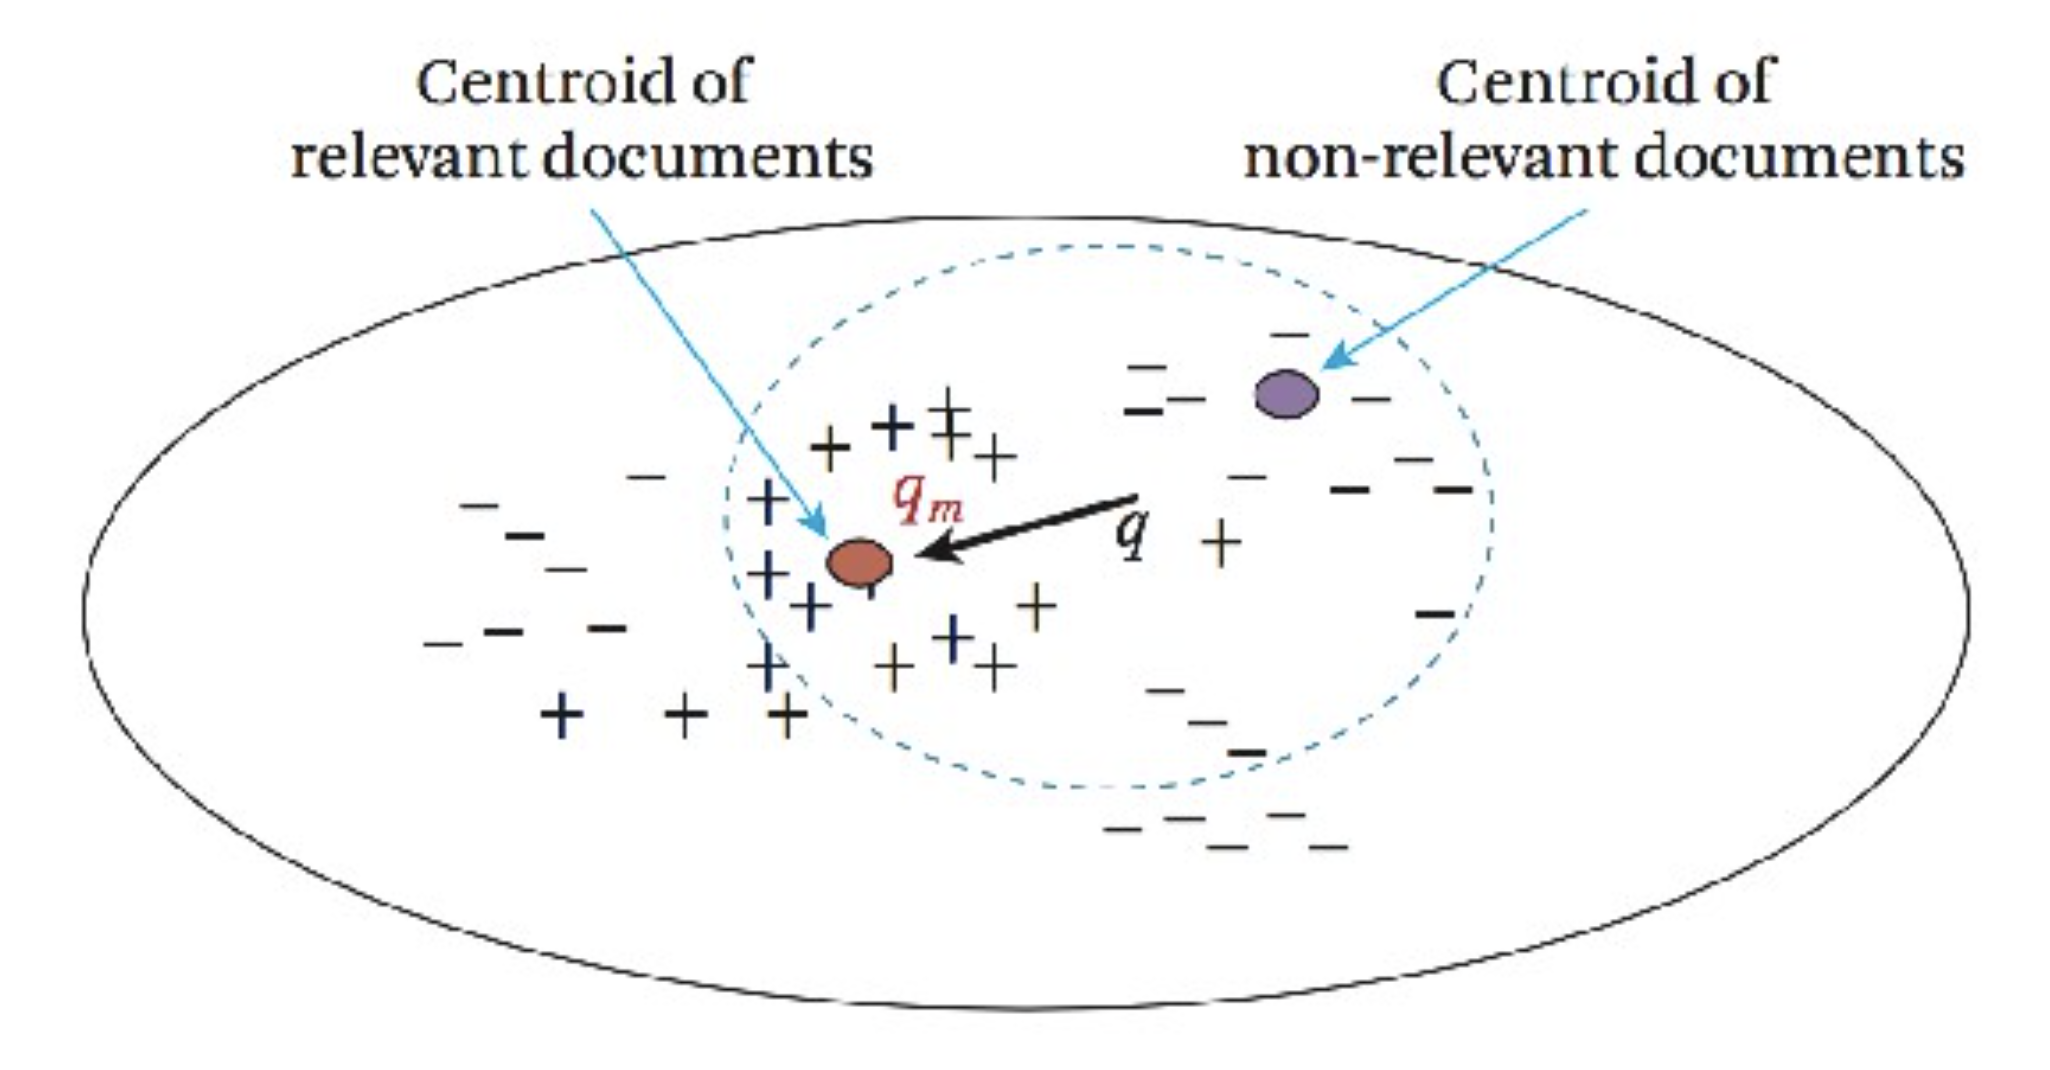
\includegraphics[width=9cm]{rocchio.png}
\end{center}
The Rocchio algorithm was invented in 1971 and revolves around the concept of an \textbf{optimal query}. The optimal query maximises the difference between the average vector representing the relevant documents and the average vector representing the non-relevant documents. \\ \\
The modified query results in a longer expanded query. This is because the terms that occur frequently in the relevant documents will be added to the modified query and those that occur frequently in non-relevant documents will be removed. \\ \\
The Rocchio feedback formula is the following:
\[ q'_j = \alpha \cdot q_j + \beta \cdot \frac{1}{|R|} \cdot \sum_{D_i \in R} d_{ij} - \gamma \cdot \frac{1}{|NR|} \cdot \sum_{D_i \in NR} d_{ij} \]
Where $\alpha$ is a constant of value 8, $\beta$ is a constant of value 16, $\gamma$ is a constant of value 4, \textit{R} is the group of relevant documents -- $|R|$ is the size of that group, and \textit{NR} is the group of non-relevant groups -- $|NR|$ is the size of that group.

\end{document}






























